\section{Introduction}
\label{sec:introduction}

% state the learning objective 
The objective of this laboratory assignment is to choose the dimensions and implement a BandPass Filter (BPF) with the a central frequency of 1kHz and a gain of 40dB (at central frequency). \par
\vspace{0.5cm}
The components used:\par
– One 741 OPAMP; \par
– At most three 1k$\Omega$ resistors; \par
– At most three 10k$\Omega$  resistors; \par
– At most three 100k$\Omega$  resistors; \par
– At most three 220nF capacitors;\par
– At most three 1$\mu$ F capacitors; \par
\vspace{0.5cm}
The bandpass filter was simulated using Ngspice, based on the script given, using the provided OPAMP model. This simulation is design to measure the output voltage gain in the passband, the central frequency and the input and output impedances at this frequency. \par
The merit was then worked on with some modifications. \par
The merit is calculated using: \par
\begin{equation}
    M = \frac{1}{Cost \times (gain_{deviation} + CentralFrequency_{deviation} + 10^{-6})}
\end{equation}\par
Where:\par
- cost = cost of resistors + cost of capacitors + cost of transistors; \par
– cost of resistors = 1 monetary unit (MU) per kOhm; \par
– cost of capacitors = 1 MU/$\mu$ F; \par
– cost of transistors = 0.1 MU per transistor; \par
\vspace{0.5cm}
Using octave, both the gain, input and the output impedances were computed at the central frequency, since we were analysing a BandPass Filter. \par
Frequency response $V_{o}(f)/V_i{f}$ was also computed, using the incremental analysis, solving the circuit for a frequency vector in log scale with 10 points per decade, from 10Hz to 100MHz.\par
\par In this assignment, the merit obtained is around $3.3 \cdot 10^{-6}$, the central frequency is 718Hz, with a gain of 34dB. Not the best values, but close to the objective, while allowing for a great learning experience.\par

It was used an incremental method in order to improve the figure of merit. Starting with a simple circuit and continuously updating it. The final circuit is shown bellow (Fig.\ref{fig:circuito}): \par

\begin{figure}[H]
\centering
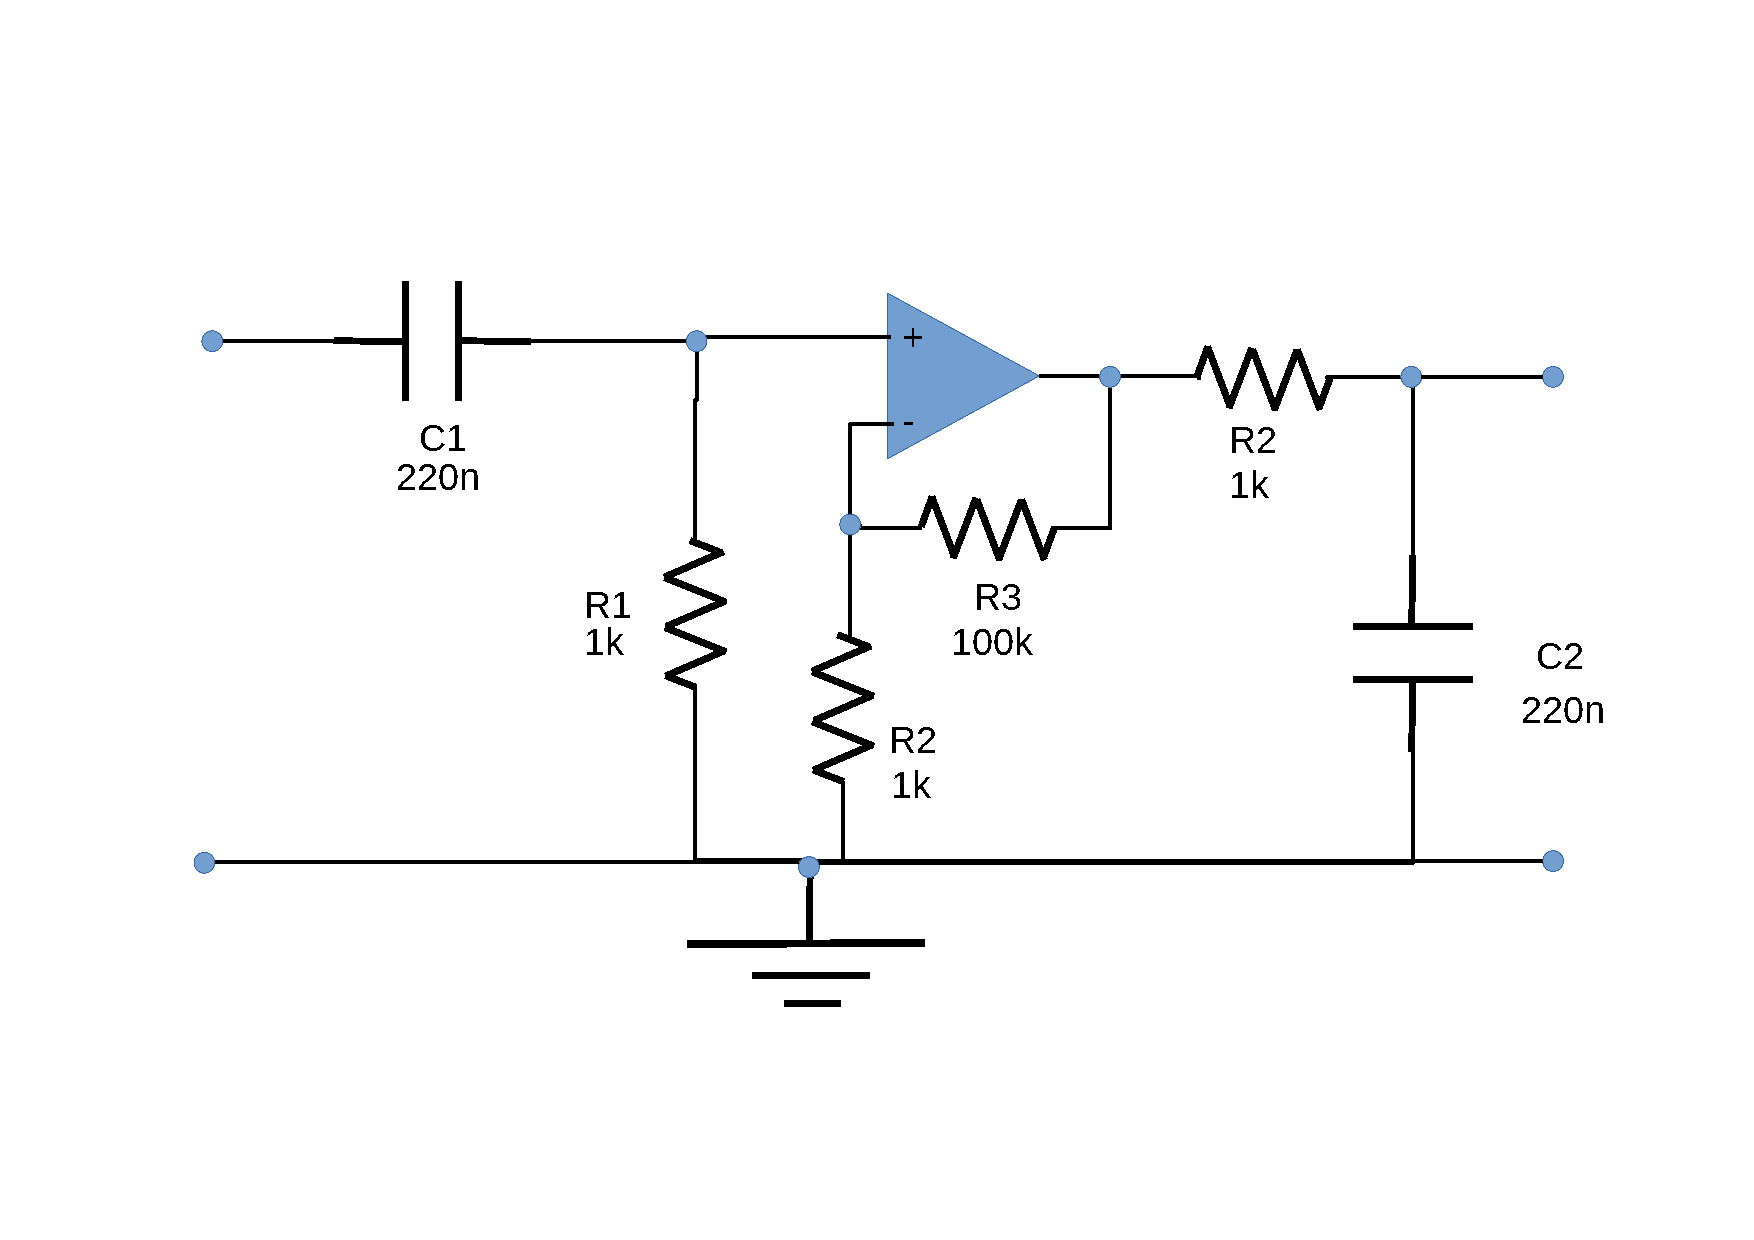
\includegraphics[width=0.9\linewidth]{circuito}
\caption{Final circuit}
\label{fig:circuito}
\end{figure}

The individual costs of the components used: 

\begin{center}
  \begin{tabular}{ | c | c | }
    \hline    
    {\bf Name} & {\bf Value} \\ \hline
    $R$ & 103k$\Omega$ \\ \hline 
    $C$ & 0.440 $\mu$S \\ 
    \hline
  \end{tabular}
  \captionof{figure}{Costs}
\end{center}

\newpage